% ----- ab hier eigentlicher Inhalt -------------------------------------------

\section{Wdh.: Gerichtete Gr.}
\subsection*{}
\begin{frame}
	\frametitle{Gerichteter Graph}
	\begin{block}{Definition}
	Ein gerichteter Graph $G$ ist ein Tupel $G=(V,E)$ mit
	\begin{itemize}
		\item der Grundmenge $V = \{v_i\}$ (die Menge der Ecken)
		\item der Relation $E\subseteq V\times V$ (die Menge der Kanten) \\ Notationen für Kanten:
		\begin{itemize}
			\item $(v,v')\in E$
			\item $v\rightarrow_G v'$
			\item $v \to v'$
		\end{itemize}
	\end{itemize}
	\end{block}
\end{frame}

\begin{frame}
	\begin{columns}
	\column{.5\textwidth}
		\begin{center}
		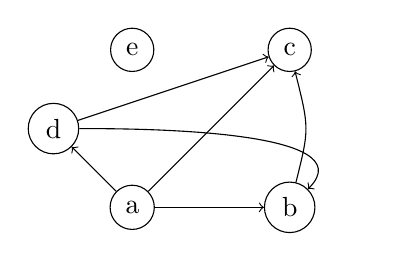
\begin{tikzpicture}
		  \tikzstyle{every node}=[draw,shape=circle];
			\path[fill] (0,0)  node[circle] (a) {a};
			\path[fill] (2,0)  node[circle] (b) {b};
			\path[fill] (2,2)  node[circle] (c) {c};
			\path[fill] (-1,1) node[circle] (d) {d};
			\path[fill] (0,2)  node[circle] (e) {e};

			\path[->,draw] (a) -- (b);
			\path[->,draw] (a) -- (d);
			\path[->,draw] (d) .. controls (0,1) and (3,1) .. (b);
			\path[->,draw] (b) .. controls (2.25,1) ..  (c);
			\path[->,draw] (a) -- (c);
			\path[->,draw] (d) -- (c);
		\end{tikzpicture}
		\end{center}
	\column{.5\textwidth}
		\begin{center}
		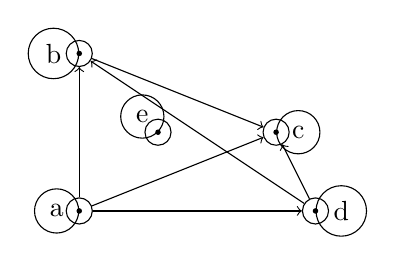
\begin{tikzpicture}
			\path[fill] (0,0)  node[circle] (a) {} node[left] {a} circle (1pt);
			\path[fill] (0,2)  node[circle] (b) {} node[left] {b} circle (1pt);
			\path[fill] (2.5,1)  node[circle] (c) {} node[right] {c} circle (1pt);
			\path[fill] (3,0) node[circle] (d) {} node[right] {d} circle (1pt);
			\path[fill] (1,1)  node[circle] (e) {} node[above left] {e} circle (1pt);

			\path[->,draw] (a) -- (b);
			\path[->,draw] (a) -- (d);
			\path[->,draw] (d) -- (b);
			\path[->,draw] (b) -- (c);
			\path[->,draw] (a) -- (c);
			\path[->,draw] (d) -- (c);
		\end{tikzpicture}
		\end{center}
	\end{columns}

	\vspace{1ex}
	\only<1>{Sind die beiden Graphen isomorph?}
	\only<2->{Ja, die beiden Graphen sind isomorph.}

	\vspace{2ex}
	\only<1>{Gebt die Graphen in Tupelschreibweise an!}
	\only<2>{Gebt den Graph in Tupelschreibweise an!}
	\only<3->{$G = ( \{a,b,c,d,e\}, \{(a,b),(a,c),(a,d),(b,c),(d,b),(d,c)\})$}
\end{frame}


\begin{frame}
	\frametitle{Graphen}
	\begin{block}{Begriffe}
		\begin{itemize}
			\item Ein Graph heißt \textbf{endlich}, wenn $V$ endlich ist ($|V|<\infty$).\pause
			\item 2 Knoten x und y heißen \textbf{adjazent}, wenn es eine Kante $(x,y)\in E$ gibt.\pause
			\item Eine \textbf{Schlinge} ist eine Kante der Form $(x,x)\in E$.\pause
			\item Ein Graph heißt \textbf{schlingenfrei}, wenn er keine Schlingen besitzt.\pause
			\item $G'=(V',E')$ ist ein \textbf{Teilgraph} von $G=(V,E)$, wenn $V'\subseteq V$ und $E'\subseteq E \cap V'\times V'$
			\item zwei Graphen sind isomorph, wenn es eine Bijektion der Knoten von $G_1$ gibt, so dass er mit $G_2$ identisch ist
		\end{itemize}
	\end{block}
\end{frame}

\begin{frame}
	\frametitle{Aufgabe}
	\begin{block}{Aufgabe}
		Gegeben sei ein gerichteter Graph mit n Knoten.
		\begin{itemize}
			\item Wieviele Kanten kann er maximal haben, wenn Schlingen erlaubt sind? \visible<2->{\textbf{Lösung:} $n^2$ Kanten}\pause
			\item Wieviele Kanten kann er maximal haben, wenn er schlingenfrei ist? \visible<3->{\textbf{Lösung:} $n(n-1)$ Kanten}
		\end{itemize}
	\end{block}
\end{frame}

\begin{frame}
	\frametitle{gerichtete Bäume}
	\begin{block}{Definition}
    In einem gerichteten Baum \ldots \pause
		\begin{itemize}
			\item  \ldots gibt es genau einen Knoten $r\in V$ so dass: \\
				für alle $x\in V$ ex. genau ein Pfad von $r$ nach $x$ \pause
			\item \ldots ist die Wurzel eindeutig
		\end{itemize}
	\end{block}
\end{frame}

\begin{frame}
	\frametitle{Pfade}
	\begin{block}{Definition}
		Ein Pfad ist eine nichtleere Liste $p=(v_0,\ldots ,v_n)\in V^+$, wenn für alle $i \in {\mathbb G}_n$ gilt $(v_i,v_{i+1})\in E$ \pause
		\begin{itemize}
			\item Die Anzahl $n=|p|-1$ (der Kanten!) heißt die \emph{Länge} des Pfades \pause
			\item Ein Pfad heißt \emph{wiederholungsfrei}, wenn alle Knoten $v_0,\ldots ,v_{n-1}$ und $v_1,\ldots ,v_n$ je paarweise verschieden sind, also maximal $v_0$ und $v_n$ gleich sind. \pause
			\item Falls $v_0=v_n$ heißt der Pfad \emph{geschlossen}. Dann ist der Pfad auch ein Zyklus.\pause
			\item ein geschlossener und wiederholungsfreier Pfad ist ein \emph{einfacher Zyklus}.
		\end{itemize}
	\end{block}
\end{frame}

\section{Wdh.: Ungerichtete Gr.}

\subsection*{}
\begin{frame}
	\frametitle{Ungerichteter Graph}
	\begin{block}{Definition}
		Ein ungerichteter Graph ist definiert als $U=(V,E)$, wobei
		\begin{itemize}
			\item $V = \{v_i\}$ die Menge der Ecken ist und
			\item $E\subseteq \{ \{x,y\}|x\in V \land y\in V\}$ die Menge der Kanten.
		\end{itemize}
	\end{block}

	\begin{center}
	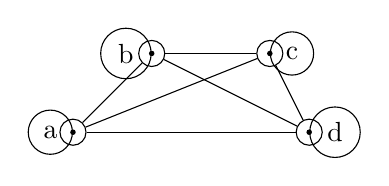
\begin{tikzpicture}
		\path[fill] (0,0)  node[circle] (a) {} node[left] {a} circle (1pt);
		\path[fill] (1,1)  node[circle] (b) {} node[left] {b} circle (1pt);
		\path[fill] (2.5,1)  node[circle] (c) {} node[right] {c} circle (1pt);
		\path[fill] (3,0) node[circle] (d) {} node[right] {d} circle (1pt);

		\path[draw] (a) -- (b);
		\path[draw] (a) -- (d);
		\path[draw] (d) -- (b);
		\path[draw] (b) -- (c);
		\path[draw] (a) -- (c);
		\path[draw] (d) -- (c);
	\end{tikzpicture}
	\\
	\vspace{1ex}
	\only<2->{Wie sähe dieser ungerichtete Graph als Menge aus?\\}
	\only<3->{$G = ( \{a,b,c,d\}, \{\{a,b\},\{a,c\},\{a,d\},\{b,c\},\{d,b\},\{d,c\}\})$}

	\end{center}
\end{frame}

\begin{frame}
	\frametitle{Aufgabe}
	\begin{block}{Aufgabe}
		Gegeben sei ein ungerichteter Graph mit n Knoten.
		\begin{itemize}
			\item Wieviele Kanten kann er maximal haben, wenn er schlingenfrei ist? \visible<2->{\textbf{Lösung:} $n(n-1)/2$ Kanten}\pause
			\item Wieviele Kanten kann er maximal haben, wenn Schlingen erlaubt sind? \visible<3->{\textbf{Lösung:} $n(n+1)/2$ Kanten}
		\end{itemize}
	\end{block}
\end{frame}

\begin{frame}
	\frametitle{zusammenhängende Graphen}
	\begin{block}{Definition}
    	Wir nennen \ldots
		\begin{itemize}
			\item einen gerichteten Graphen \emph{streng zusammenhängend},
				wenn für jedes Knotenpaar $(x,y)\in V^2$ gilt: Es gibt in $G$ einen Pfad von $x$ nach $y$.\\ \pause
			\item einen ungerichteten Graphen \emph{zusammenhängend}, wenn der entsprechende gerichtete Graph \emph{streng zusammenhängend} ist.
		\end{itemize}
	\end{block}
\end{frame}

\begin{frame}
	\frametitle{ungerichtete Bäume}
	\begin{block}{Definition}
		\begin{itemize}
			\item Jeder zusammenhängende ungerichtete Graph mit $|E| = |V| - 1$ ist ein ungerichteter Baum \pause
			\item Im ungerichteten Baum kann theoretisch jeder Knoten Wurzel sein. \\ \pause
			\item Daher wird i.d.R. ein Knoten als Wurzel hervorgehoben.
		\end{itemize}
	\end{block}
\end{frame}


\section{Gewichtete Graphen}
\subsection*{}
\begin{frame}
\frametitle{Maximaler Fluss eines Graphen}

	\begin{block}{Allgemein}
		\begin{itemize}
          \item Gegeben ein Graph, dessen Kanten durch $c(u,v)$ gewichtet sind \pause
          \item Der Graph besitze einen ausgezeichneten Anfangsknoten(Quelle)
          und Endknoten(Senke) \pause
          \item Gesucht ist der maximale Fluss zwischen Quelle und Senke
          \end{itemize}
	\end{block}
\pause
	\begin{block}{Beispiel}
		Gegeben sei ein Rohrsystem (von q nach s), durch das Wasser fließt. Wie viel
		Wasser kann auf einmal durch das Rohrsystem fließen?
	\end{block}
\end{frame}

\begin{frame}
\frametitle{Beispielgraph}
	\begin{center}
		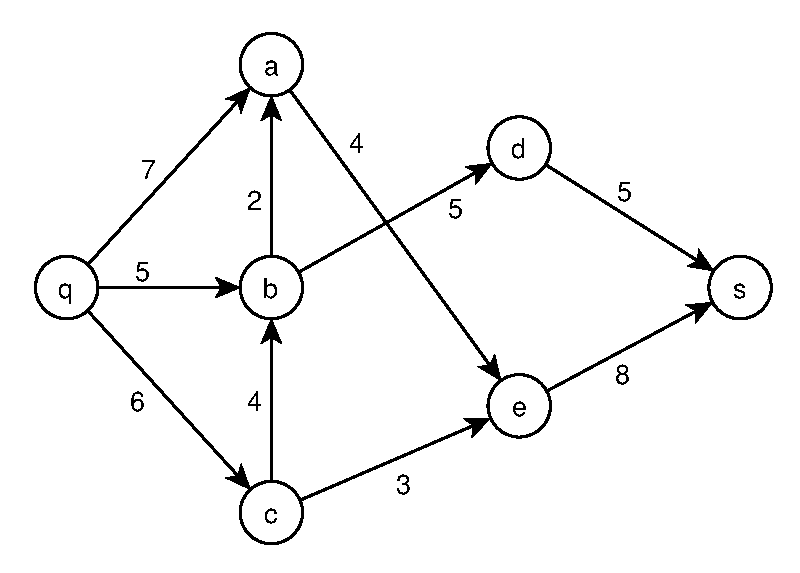
\includegraphics[width=11cm,
		height=7cm,keepaspectratio=true]{src/tut07_fluss_1}
	\end{center}
\end{frame}

\begin{frame}
\frametitle{Beispiel Routenplanung}
	\begin{block}{Beispiel}
		Was ist der kürzeste Weg von S nach Z wenn an den Kanten die Entfernung zwischen den Städten eingetragen ist?
	\end{block}
\end{frame}

\section*{Matrizen}

\begin{frame}
	\frametitle{Matrizenrechnen!}
		\large Wer wünscht sich dazu Beispiele?
\end{frame}


\section{Darstellungsformen}
\subsection*{}
\begin{frame}
\frametitle{Graphen im Rechner}
		\begin{center}
			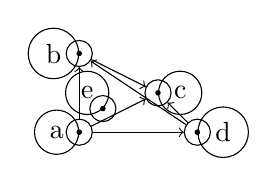
\begin{tikzpicture}
				\path[fill] (0,0)  node[circle] (a) {} node[left] {a} circle (1pt);
				\path[fill] (0,1)  node[circle] (b) {} node[left] {b} circle (1pt);
				\path[fill] (1,0.5)  node[circle] (c) {} node[right] {c} circle (1pt);
				\path[fill] (1.5,0) node[circle] (d) {} node[right] {d} circle (1pt);
				\path[fill] (0.3,0.3)  node[circle] (e) {} node[above left] {e} circle (1pt);

				\path[->,draw] (a) -- (b);
				\path[->,draw] (a) -- (d);
				\path[->,draw] (d) -- (b);
				\path[->,draw] (b) -- (c);
				\path[->,draw] (a) -- (c);
				\path[->,draw] (d) -- (c);
			\end{tikzpicture}
		\end{center}

		\begin{block}{Ein Graph - verschiedene Schreibweisen}
			Für den oben angegebenen Graphen - in grafischer Darstellung - gibt es verschiedene Darstellungsarten:
			\begin{description}
				\only<-1>{
					\item[\xb{Tupeldarstellung}] (aus dem letzten Tut):\\
					$G = ( \{a,b,c,d,e\},$\\
					$\{(a,b),(a,c),(a,d),(b,c),(d,b),(d,c)\})$
				}
				\only<2>{
					\item[\xb{Adjazenzliste}]: 	\\
										a: [b,c,d]\\
										b: [c]\\
										c: []\\
										d: [b, c]\\
										e: []
				}
				\only<3->{
					\item[\xb{Adjazenzmatrix}]
							$A =$ $\left(
							\begin{matrix}
							0 & 1 & 1 & 1 & 0\\
							0 & 0 & 1 & 0 & 0\\
							0 & 0 & 0 & 0 & 0\\
							0 & 1 & 1 & 0 & 0\\
							0 & 0 & 0 & 0 & 0
							\end{matrix}
							\right)$
				}	\only<4->{
					 was bedeutet $(A^2)_{ij}$ ?
				}
			\end{description}
		\end{block}
\end{frame}

\begin{frame}
\frametitle{Liste vs. Matrix}
	\begin{block}{Adjazenzlisten}
	\begin{itemize}
		\visible<2->{\item einfacher Zugriff auf alle adjazenten Knoten}
		\visible<3->{\item Um zu überprüfen, ob eine Kante existiert, muss man eventuell alle Nachbarn durchgehen}
	\end{itemize}
	\end{block}

	\begin{block}{Adjanzenzmatrixen}
	\begin{itemize}
		\visible<4->{\item schnelle Überprüfung, ob eine Kante zwischen zwei Knoten $i$ und $j$ existiert}
		\visible<5->{\item Um auf einen Nachbarn zuzugreifen, muss man eventuell alle Knoten durchgehen}
	\end{itemize}
	\end{block}
\end{frame}
\begin{frame}
\frametitle{Liste vs. Matrix}
	\begin{block}{Welche Darstellungsform ist geeigneter?}
		Für einen...
		\begin{itemize}
			\visible<1->{\item vollständigen Graphen? \visible<2->{\\Adjazenzmatrix}}\pause
			\item Graphen mit nur wenigen Kanten? \visible<3->{\\Adjazenzliste}\pause
			\item Graphen, den wir später auf Reflexivität untersuchen wollen? \visible<4->{\\Adjazenzmatrix}
		\end{itemize}
	\end{block}
\end{frame}

\section{Wegematrix}
\begin{frame}
	\frametitle{Wegematrix I}
	\begin{block}{Darstellung von Relationen}
		So wie die Adjazenzmatrix Relationen zwischen Knoten darstellt, können auch weitere Relationen als Matrix dargestellt werden. Ein Beispiel ist die Wegematrix, die eine Darstellungsform der Erreichbarkeitssrelation
		$E^*=\bigcup^{n-1}_{i=0} E^i $. \\
	\end{block}
	\begin{block}{Für die Wegematrix gilt}
 \begin{displaymath}
 W_{ij}=
	\begin{cases}
		1, & \text{falls es in G einen Pfad von i nach j gibt} \\
		0, & \text{falls es in G keinen Pfad von i nach j gibt}
	\end{cases}
	\end{displaymath}
	\end{block}
\end{frame}

\subsection{Algorithmen}
\begin{frame}
	\frametitle{Aufwand}
	\begin{block}{Zählweise}
		Beim Vergleich verschiedener Algorithmen in Bezug auf den Aufwand, sucht man nach einem Maß für die Anzahl der Rechenoperationen für eine Aufgabe der Größe $n$.
	\end{block}
	\begin{block}{Beispiel} \pause
		Summe aller Zahlen von $1$ bis $n$: \\

			$\sum^n_{i=0} i = $\pause$n*(n+1)/2$

	\end{block}
\end{frame}

\begin{frame}
	\frametitle{Algorithmus I}
% 	\begin{block}{einfacher Algorithmus zur Wegematrix}
% \end{block}

\lstinputlisting{src/tut07_algo1.txt}

\end{frame}

\begin{frame}
	\frametitle{Algorithmus II}
% 	\begin{block}{einfacher Algorithmus zur Wegematrix}
% \end{block}

\lstinputlisting{src/tut07_algo2.txt}

\end{frame}

%
%% Der folgende Worsch-Tex will nicht funktionieren:
\begin{frame}
	\frametitle {Wegematrix II}
	\begin{columns}
		\column{.5\textwidth}
		\begin{center}
		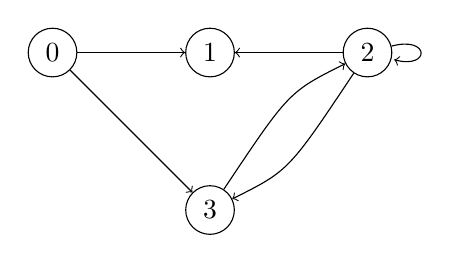
\begin{tikzpicture}
		  \tikzstyle{every node}=[draw,shape=circle];
			\path[fill] (0,0)  node[circle] (0) {0};
			\path[fill] (2,0)  node[circle] (1) {1};
			\path[fill] (4,0)  node[circle] (2) {2};
			\path[fill] (2,-2) node[circle] (3) {3};

			\path[->,draw] (0) -- (1);
			\path[->,draw] (2) -- (1);
			\path[->,draw] (2) edge [loop right] ();
			\path[->,draw] (3) .. controls (3,-0.5) ..  (2);
			\path[->,draw] (2) .. controls (3,-1.5) ..  (3);
			\path[->,draw] (0) -- (3);
		\end{tikzpicture}
		\end{center}
    \column{.5\textwidth}
				$\left(
						\begin{matrix}
							0 & 1 & 0 & 1 \\
							0 & 0 & 0 & 0 \\
							0 & 1 & 1 & 1 \\
							0 & 0 & 1 & 0
						\end{matrix}
				\right)$
	\end{columns}
	\begin{block}{Ihr seid dran...}
		\begin{itemize}
			\item Wie sieht die Wegematrix zum oben gezeigten Graph aus?
			\visible<2->{\item Wie sieht die Wegematrix für eine vollständig mit 1en gefüllte Matrix aus?}
			\visible<3->{\item Wann gilt allgemein $W=A$? Wann gilt $E^1=A$?}
		\end{itemize}
	\end{block}
\end{frame}


\section{Warshall-Algorithmus}
\subsection*{}
\begin{frame}
	\frametitle{Reflexive Transitive Hülle nach Warshall}

	Gegeben sei eine reflexive Relation $\rho$ über einer endlichen Eckenmenge $E=\{0,\dots,n-1\}$.
	$\sigma^{(k)}$ sei folgende Relation:
	\begin{multline*}
		\sigma^{(k)} = \{(i,j)\in E \times E | \exists \text{Weg } i \to e_1 \to \cdots \to e_{l-1} \to j \\
		\text{ mit } l\le k+2, e_r\in\{0,\ldots,k\} \text{ für } 1\le r\le l-1\}
	\end{multline*}

	\begin{columns}
	\column{.2\textwidth}
		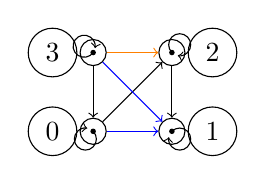
\begin{tikzpicture}
			\path[fill] (0,0)  node[circle] (0) {} node[left=2mm] {0} circle (1pt);
			\path[fill] (1,0)  node[circle] (1) {} node[right=2mm] {1} circle (1pt);
			\path[fill] (1,1)  node[circle] (2) {} node[right=2mm] {2} circle (1pt);
			\path[fill] (0,1)  node[circle] (3) {} node[left=2mm] {3} circle (1pt);

			\path[->,draw] (0) arc(45:-280:1.4mm);
			\path[->,draw] (1) arc(135:-190:1.4mm);
			\path[->,draw] (2) arc(225:-100:1.4mm);
			\path[->,draw] (3) arc(325:-10:1.4mm);
			\path[->,draw] (3) -- (0);
			\path[->,draw] (0) -- (2);
			\path[->,draw] (2) -- (1);
			\visible<2->{\path[->,draw,orange] (3) -- (2);}
			\visible<6->{\path[->,draw,blue] (3) -- (1);}
			\visible<6->{\path[->,draw,blue] (0) -- (1);}
		\end{tikzpicture}
	\column{.4\textwidth}
		\[
		{\color{orange} \sigma^{(0)}}:\
		\alt<2->{
			\left(
			\begin{matrix}
			1 & 0 & 1 & 0\\
			0 & 1 & 0 & 0\\
			0 & 1 & 1 & 0\\
			1 & 0 & {\color{orange}1} & 1
			\end{matrix}
			\right)
		}{
			\left(
			\begin{matrix}
			1 & 0 & 1 & 0\\
			0 & 1 & 0 & 0\\
			0 & 1 & 1 & 0\\
			1 & 0 & 0 & 1
			\end{matrix}
			\right)
		}
		\]
		\[
		\visible<5->{
			{ \color{blue} \sigma^{(2)}}:\
		}
		\alt<-5>{
			\visible<5->{
				\left(
				\begin{matrix}
				1 & 0 & 1 & 0\\
				0 & 1 & 0 & 0\\
				0 & 1 & 1 & 0\\
				1 & 0 & {\color{orange}1} & 1
				\end{matrix}
				\right)
			}
		}
		{
			\left(
			\begin{matrix}
			1 & {\color{blue} 1} & 1 & 0\\
			0 & 1 & 0 & 0\\
			0 & 1 & 1 & 0\\
			1 & {\color{blue} 1} & {\color{orange}1} & 1
			\end{matrix}
			\right)
		}
		\]
	\column{.4\textwidth}
		\[
		\visible<3->{
			{ \color{green} \sigma^{(1)}}:\
		}
		\alt<-3>{
			\visible<3->{
				\left(
				\begin{matrix}
				1 & 0 & 1 & 0\\
				0 & 1 & 0 & 0\\
				0 & 1 & 1 & 0\\
				1 & 0 & {\color{orange}1} & 1
				\end{matrix}
				\right)
			}
		}
		{
			\left(
			\begin{matrix}
			1 & 0 & 1 & 0\\
			0 & 1 & 0 & 0\\
			0 & 1 & 1 & 0\\
			1 & 0 & {\color{orange}1} & 1
			\end{matrix}
			\right)
		}
		\]
		\[
		\visible<7->{
			{ \color{red} \sigma^{(3)}}:\
		}
		\alt<-7>{
			\visible<7->{
				\left(
				\begin{matrix}
				1 & {\color{blue} 1} & 1 & 0\\
				0 & 1 & 0 & 0\\
				0 & 1 & 1 & 0\\
				1 & {\color{blue} 1} & {\color{orange}1} & 1
				\end{matrix}
				\right)
			}
		}
		{
			\left(
			\begin{matrix}
			1 & {\color{blue} 1} & 1 & 0\\
			0 & 1 & 0 & 0\\
			0 & 1 & 1 & 0\\
			1 & {\color{blue} 1} & {\color{orange}1} & 1
			\end{matrix}
			\right)
		}
		\]
	\end{columns}
\end{frame}


\begin{frame}[fragile]
	\frametitle{Der Warshall-Algorithmus}

	\begin{block}{Anforderungsbeschreibung}
		\begin{description}
			\item[Eingabe:]Adjazenzmatrix $A$ einer Relation $\sigma$
			\item[Ausgabe:] Adjanzenzmatrix $S$ von $\sigma^*$ \pause (entspricht der
			Erreichbarkeitsrelation)
		\end{description}
	\end{block}

	\pause
	\begin{block}{Der Algorithmus}
		\begin{lstlisting}[language = Java,mathescape,morekeywords={set}]
	$S$ := $A$
 for $i=0,\ldots,n-1$ set $s_{ii}$ := $1$

 for $k=0,\ldots,n-1$
   for $i=0,\ldots, n-1$
     for $j=0,\ldots, n-1$
       if ($s_{ij}$ + $s_{ik}$ * $s_{kj}$) >= 1 set $s_{ij}$ := 1
		\end{lstlisting}
	\end{block}
\end{frame}



\section{Abschluss}
% Studis anzuregen darüber nachzudenken, ob sie wirklich alles wissen, ansonsten nachlesen oder fragen nachträglich stellen, dann kann in der nächsten Woche nochmal drauf eingegangen werden
\subsection*{}
\begin{frame}
	\frametitle{Zum Schluss...}
	\begin{block}{Was ihr nun wissen solltet!}
	\begin{itemize}
	  	\visible<2->{\item Begriffe: Adjazent, Schlinge, Pfad, Zyklus, $\ldots$?}
		\visible<3->{\item Wie werden Graphen im Rechner dargestellt?}
		\visible<4->{\item Vor- \& Nachteile von Adjazenzliste und Adjazenzmatrix}
		\visible<5->{\item Was ist eine Wegematrix?}
		\visible<6->{\item Was sind Gewichte von Graphen und wozu sind sie nützlich?}
    \end{itemize}
   	\end{block}

	\visible<7->{
	\begin{block}{Ihr wisst was nicht?}
		Stellt \textbf{jetzt} Fragen!
	\end{block}}
\end{frame}
